% Figura Anexo I: la asimetría central del catálogo: pérdida privada de segundo orden, pérdida social de primer orden
\documentclass[tikz,border=3pt]{standalone}
\usepackage[T1]{fontenc}
\usepackage[utf8]{inputenc}
\usepackage{amsmath}
\usetikzlibrary{arrows.meta,calc,positioning}
\begin{document}
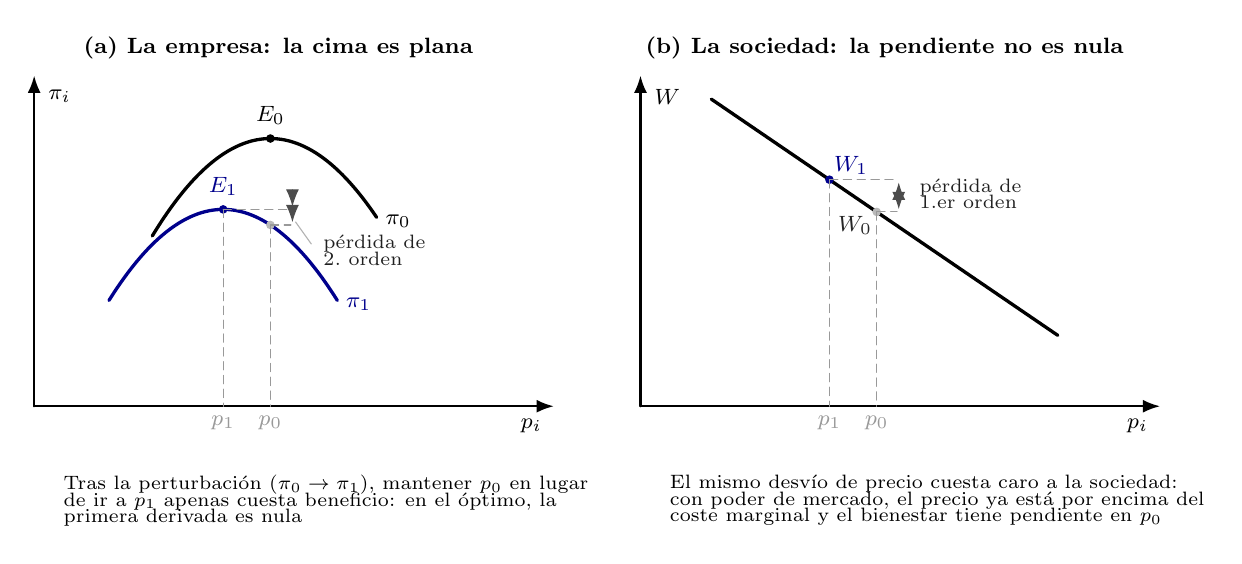
\begin{tikzpicture}[>={Latex[length=2.2mm]}, line cap=round, font=\footnotesize,
  eje/.style={->, thick},
  curva/.style={very thick},
  nueva/.style={very thick, blue!55!black},
  guia/.style={densely dashed, gray!80},
  pto/.style={circle, fill=black, inner sep=1.1pt}]
  % ---------- Panel (a): la empresa ----------
  \node[font=\footnotesize\bfseries] at (3.1,4.55) {(a) La empresa: la cima es plana};
  \draw[eje] (0,0) -- (6.6,0) node[below left=1pt]{$p_i$};
  \draw[eje] (0,0) -- (0,4.2) node[below right=2pt]{$\pi_i$};
  \draw[curva, domain=1.5:4.35, samples=60] plot (\x,{3.4-0.55*(\x-3.0)^2});
  \node[anchor=west, inner sep=1pt] at (4.42,2.35) {$\pi_0$};
  \draw[nueva, domain=0.95:3.85, samples=60] plot (\x,{2.5-0.55*(\x-2.4)^2});
  \node[anchor=west, inner sep=1pt, blue!55!black] at (3.92,1.30) {$\pi_1$};
  \node[pto] (E0) at (3.0,3.4) {};
  \node[above=2pt of E0, inner sep=1pt] {$E_0$};
  \node[pto, fill=blue!55!black] (E1) at (2.4,2.5) {};
  \node[above=2pt of E1, inner sep=1pt, blue!55!black] {$E_1$};
  \node[pto, fill=gray!55] (S) at (3.0,2.302) {};
  \draw[guia] (2.4,2.5) -- (2.4,0) node[below]{$p_1$};
  \draw[guia] (3.0,2.302) -- (3.0,0) node[below]{$p_0$};
  \draw[<->, gray!60!black, shorten >=1pt, shorten <=1pt] (3.28,2.5) -- (3.28,2.302);
  \draw[guia] (2.4,2.5) -- (3.26,2.5);
  \draw[guia] (3.0,2.302) -- (3.26,2.302);
  \node[anchor=west, font=\scriptsize, align=left, gray!25!black] at (3.55,1.98) {pérdida de\\[-2pt]$2.º$ orden};
  \draw[gray!60] (3.52,2.06) -- (3.32,2.34);
  \node[align=left, anchor=north west, font=\scriptsize] at (0.25,-0.75)
    {Tras la perturbación ($\pi_0\to\pi_1$), mantener $p_0$ en lugar\\[-2pt]de ir a $p_1$ apenas cuesta beneficio: en el óptimo, la\\[-2pt]primera derivada es nula};
  % ---------- Panel (b): la sociedad ----------
  \begin{scope}[xshift=7.7cm]
    \node[font=\footnotesize\bfseries] at (3.1,4.55) {(b) La sociedad: la pendiente no es nula};
    \draw[eje] (0,0) -- (6.6,0) node[below left=1pt]{$p_i$};
    \draw[eje] (0,0) -- (0,4.2) node[below right=2pt]{$W$};
    \draw[curva] (0.9,3.9) -- (5.3,0.9);
    \node[pto, fill=blue!55!black] (W1) at (2.4,2.877) {};
    \node[above right=-1pt of W1, inner sep=1pt, blue!55!black] {$W_1$};
    \node[pto, fill=gray!55] (W0) at (3.0,2.468) {};
    \node[below left=-1pt of W0, inner sep=1pt, gray!30!black] {$W_0$};
    \draw[guia] (2.4,2.877) -- (2.4,0) node[below]{$p_1$};
    \draw[guia] (3.0,2.468) -- (3.0,0) node[below]{$p_0$};
    \draw[<->, gray!60!black, shorten >=1pt, shorten <=1pt] (3.28,2.877) -- (3.28,2.468);
    \draw[guia] (2.4,2.877) -- (3.26,2.877);
    \draw[guia] (3.0,2.468) -- (3.26,2.468);
    \node[anchor=west, font=\scriptsize, align=left, gray!25!black] at (3.42,2.7) {pérdida de\\[-2pt]$1.\text{er}$ orden};
    \node[align=left, anchor=north west, font=\scriptsize] at (0.25,-0.75)
      {El mismo desvío de precio cuesta caro a la sociedad:\\[-2pt]con poder de mercado, el precio ya está por encima del\\[-2pt]coste marginal y el bienestar tiene pendiente en $p_0$};
  \end{scope}
\end{tikzpicture}
\end{document}
